\section{Grundlagen}
Im den folgenden Abschnitten werden die benötigten Grundlagen gelegt, um die
im Projekt verwendeten Techniken und Algorithmen zu verstehen. An dieser Stelle
ist anzumerken, dass für detaliertes Verständnis ein Lehrbuch
wie zum Beispiel \cite{hands_on_machine_learning} studiert werden sollte.

Die verwendeten Techniken und Algorithmen werden in den Bereich \emph{Machine
Learning} eingeordnet und umfassen \emph{Neuronale Netzwerke}, \emph{Convolutional Netzwerke},
\emph{Autoencoder} und \emph{Random Forests}. All diese Techniken sind
\emph{supervised} Algorithmen also überwachte Lerner. Damit ist gemeint, dass
den Algorithmen neben den Daten auch die passende Wahrheit in Form von Labels
mit übergegeben bekommen \cite[S. 8]{hands_on_machine_learning}. Dies ist für die
Problemstellung der Hunderassenbestimmung nicht unüblich, da es hierbei um ein
klassiches Klassifizierungsproblem handelt \cite[S. 8]{hands_on_machine_learning}.

\subsection{Neuronale Netzwerke}
Die Entwicklung von künstliche neuronalen Netzwerke (NN) wurden inspiert von den
leistungsstarken biologischen neuronale Netzwerken die in ihrer Gesamtheit
das Gehirn vieler Lebewesen bilden \cite[S. 253-256]{hands_on_machine_learning}.
Zum jetzigen Zeitpunkt generalisieren NN jedoch noch nicht in der Weise
wie es ihre biologische Vorbilder tun. Damit
ist gemeint, dass viele Algorithmen nur spezifische Probleme, die sie gelernt haben,
lösen könen und bisher kaum Transferleistung erbringen können \cite{transferleistung_netzwerke}.

\subsection{Datensatz}
Wie oben angesprochen benötigen überwachte Lernern während des Traningprozesses
die Labels welche die Wahrheit über die Daten enthalten. In disem Fall wäre die
benötigte Wahrheit der Name der Hunderasse. Dementsprechen wird ein Datensatz
benötigt, der die Labels mit enthält. Selbstverständlich könnte ein Datensatz
selber erstellt und gelabelt werden, dies ist jedoch mit einer hohen Arbeitsaufwand
verknüpft. Zusätzlich enthält der Datensatz für jedes Bild Koordinaten
für einen Rahmen (Bounding Box) der den Hund enthält.

Vorteilhafterweise bietet die Internetseite \emph{kaggle} einen gelabelten
Datensatz \cite{datensatz}. Durch diesen wird maximale Anzahl von $120$
Hunderassen die klassifiziert werden soll festgelegt. Insgesamt enthält der
Datensatz $20580$ Bilder die auf die $120$ Rassen aufgeteilt ist. Wie in der
Abbildung \ref{fig:gleichverteilung_bilder} zu erkennen ist, sind die Bilder
gleichmäßig auf die einzelnen Klassen aufgeteilt.
\begin{figure}
\centering
\includegraphics[width=\the\textwidth]{../../final_data/general/image_distribution.pdf}
\caption{Bildverteilung der einzelnen Klassen. Die Namen der jeweiligen Rassen
         wurden durch Platzhalter ersetzt, weil lediglich verdeutlich werden soll
         das die Bilder gleichverteilt sind.}
\label{fig:gleichverteilung_bilder}
\end{figure}
Eine zufällig Auswahl von Bildern des Datensatzes sind in der Abbildung \ref{fig:bilder_cluser}
dargestellt.
\begin{figure}
\centering
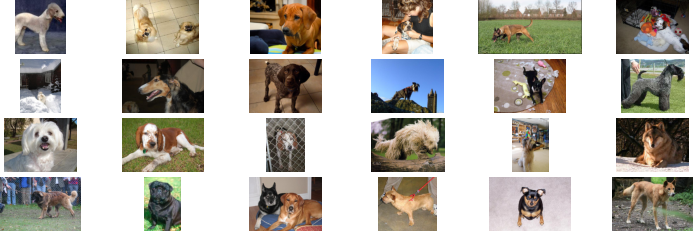
\includegraphics[width=\the\textwidth]{../../final_data/general/image_cluster.pdf}
\caption{Zufällig ausgewählte Bilder des Datensatz.}
\label{fig:bilder_cluser}
\end{figure}
Es ist deutlich zuerkennen, dass einzelne Bilder schwieriger zu klassifizieren sind,
da Menschen, Hindernisse oder andere Hunde im Bild enthalten sind. Außerdem
fältt auf, dass die Auflösung der Bilder nicht homogen ist.

\subsubsection{Verarbeitung der Daten}
Um den Datensatz für das tranieren der verschiedenen Algorithmen zu verwenden,
muss er zunächst in einen Tranings-, Validierungs- und Testdatensatz aufgeteilt
werden. Die gewählten Anteile sind $0.6-0.2-0.2$ verwendet und entspricht damit
den in der Literatur \cite[S. 29]{hands_on_machine_learning} empfohlenen Werten.

Während der Tranignsphase werden die Bilder batch-weise geladen und vorprozessiert.
Der Grund für das batch-weise laden ist, dass damit verhindert wird das $20580$
aufeinmal in den Arbeitspeicher geladen werden, was die Leistung der späteren
Traningsphase auf Grund von mangelden Ressourcen beeinträchtigen kann. Die erstellte
Datenlader (Dataloader) Klasse basiert auf der \textsc{keras.utils.Sequence} Klasse die eine
automatische Parallesierung des Ladeprozesses und der Vorverarbeitung ermöglicht
\cite{keras_sequentiel}.

Mit dem Dataloader besitzt die Funktion die Bilder batch-weise auf eine gegebene
Bildgröße runterzuskalieren. Auf die einzelnen Skalierungsgrößen wird in dem
Kapitel \ref{sec:NNarchitekturen} eingegangen, da diese nicht für alle Architekturen
gleich sind. Die batch-weise Reskalierung ist auf Grund der inhomogenität
der Bildauflösungen notwendig, weil \textsc{numpy.array}
eine feste Eingangsform (Input shape) voraussetzen, ergo eine homogene Bildauflösung
innerhalb eines Batches.

Darüber hinaus werden Techniken der \emph{Data Augementation} angewandt, um
die Statistik des Datensatz zuvergrößern. Dies ist sinnvoll, da mit durchschnittlich
$172$ Bildern pro Rassen (vgl. Abbildung \ref{fig:gleichverteilung_bilder})
bei $120$ Rassen, im Vergleich z.\,B. zu Googles \textsc{Open Image} Datensatz
\cite{google_open_image}, wenig Bilder für die Anzahl der Rassen enthält.
Ausdiesem Grund verwenden wir zufällige Rotationen, Translationen und Vergrößerungen
der Bilder, um die allgemeine Statistik zu erhöhen. Hierbei wird sichergestellt
, dass nach einer Translation oder einer Vergrößerung immernoch der ganze Hund
im Bild zu erkennen ist. Hierfür werden die im Datensatz enthaltenten Bounding
Boxes verwendet. Beispielhafte Ergebnisse der Transformationen sind in Abbildung
\ref{fig:data_augementation} dargestellt.
\begin{figure}
\centering
\includegraphics[width=\the\textwidth]{../../final_data/general/data_augementation.pdf}
\caption{Beispielhafte Transformationen.}
\label{fig:data_augementation}
\end{figure}


\section{Verwendete NN Architekturen}\label{sec:NNarchitekturen}

\subsection{5 Hunderassen}

\subsection{120 Hunderassen}
